Für die Messungen wurden im Laufe des Projekts zwei Versionen an Prototyp-Platinen entworfen. Im Verlauf der Versuche wurden Veränderungen an den Platinen vorgenommen, um den Betrieb dieser zu verbessern. 
\section{Prototyp 1}
\begin{center}
\begin{minipage}{0.75\textwidth}
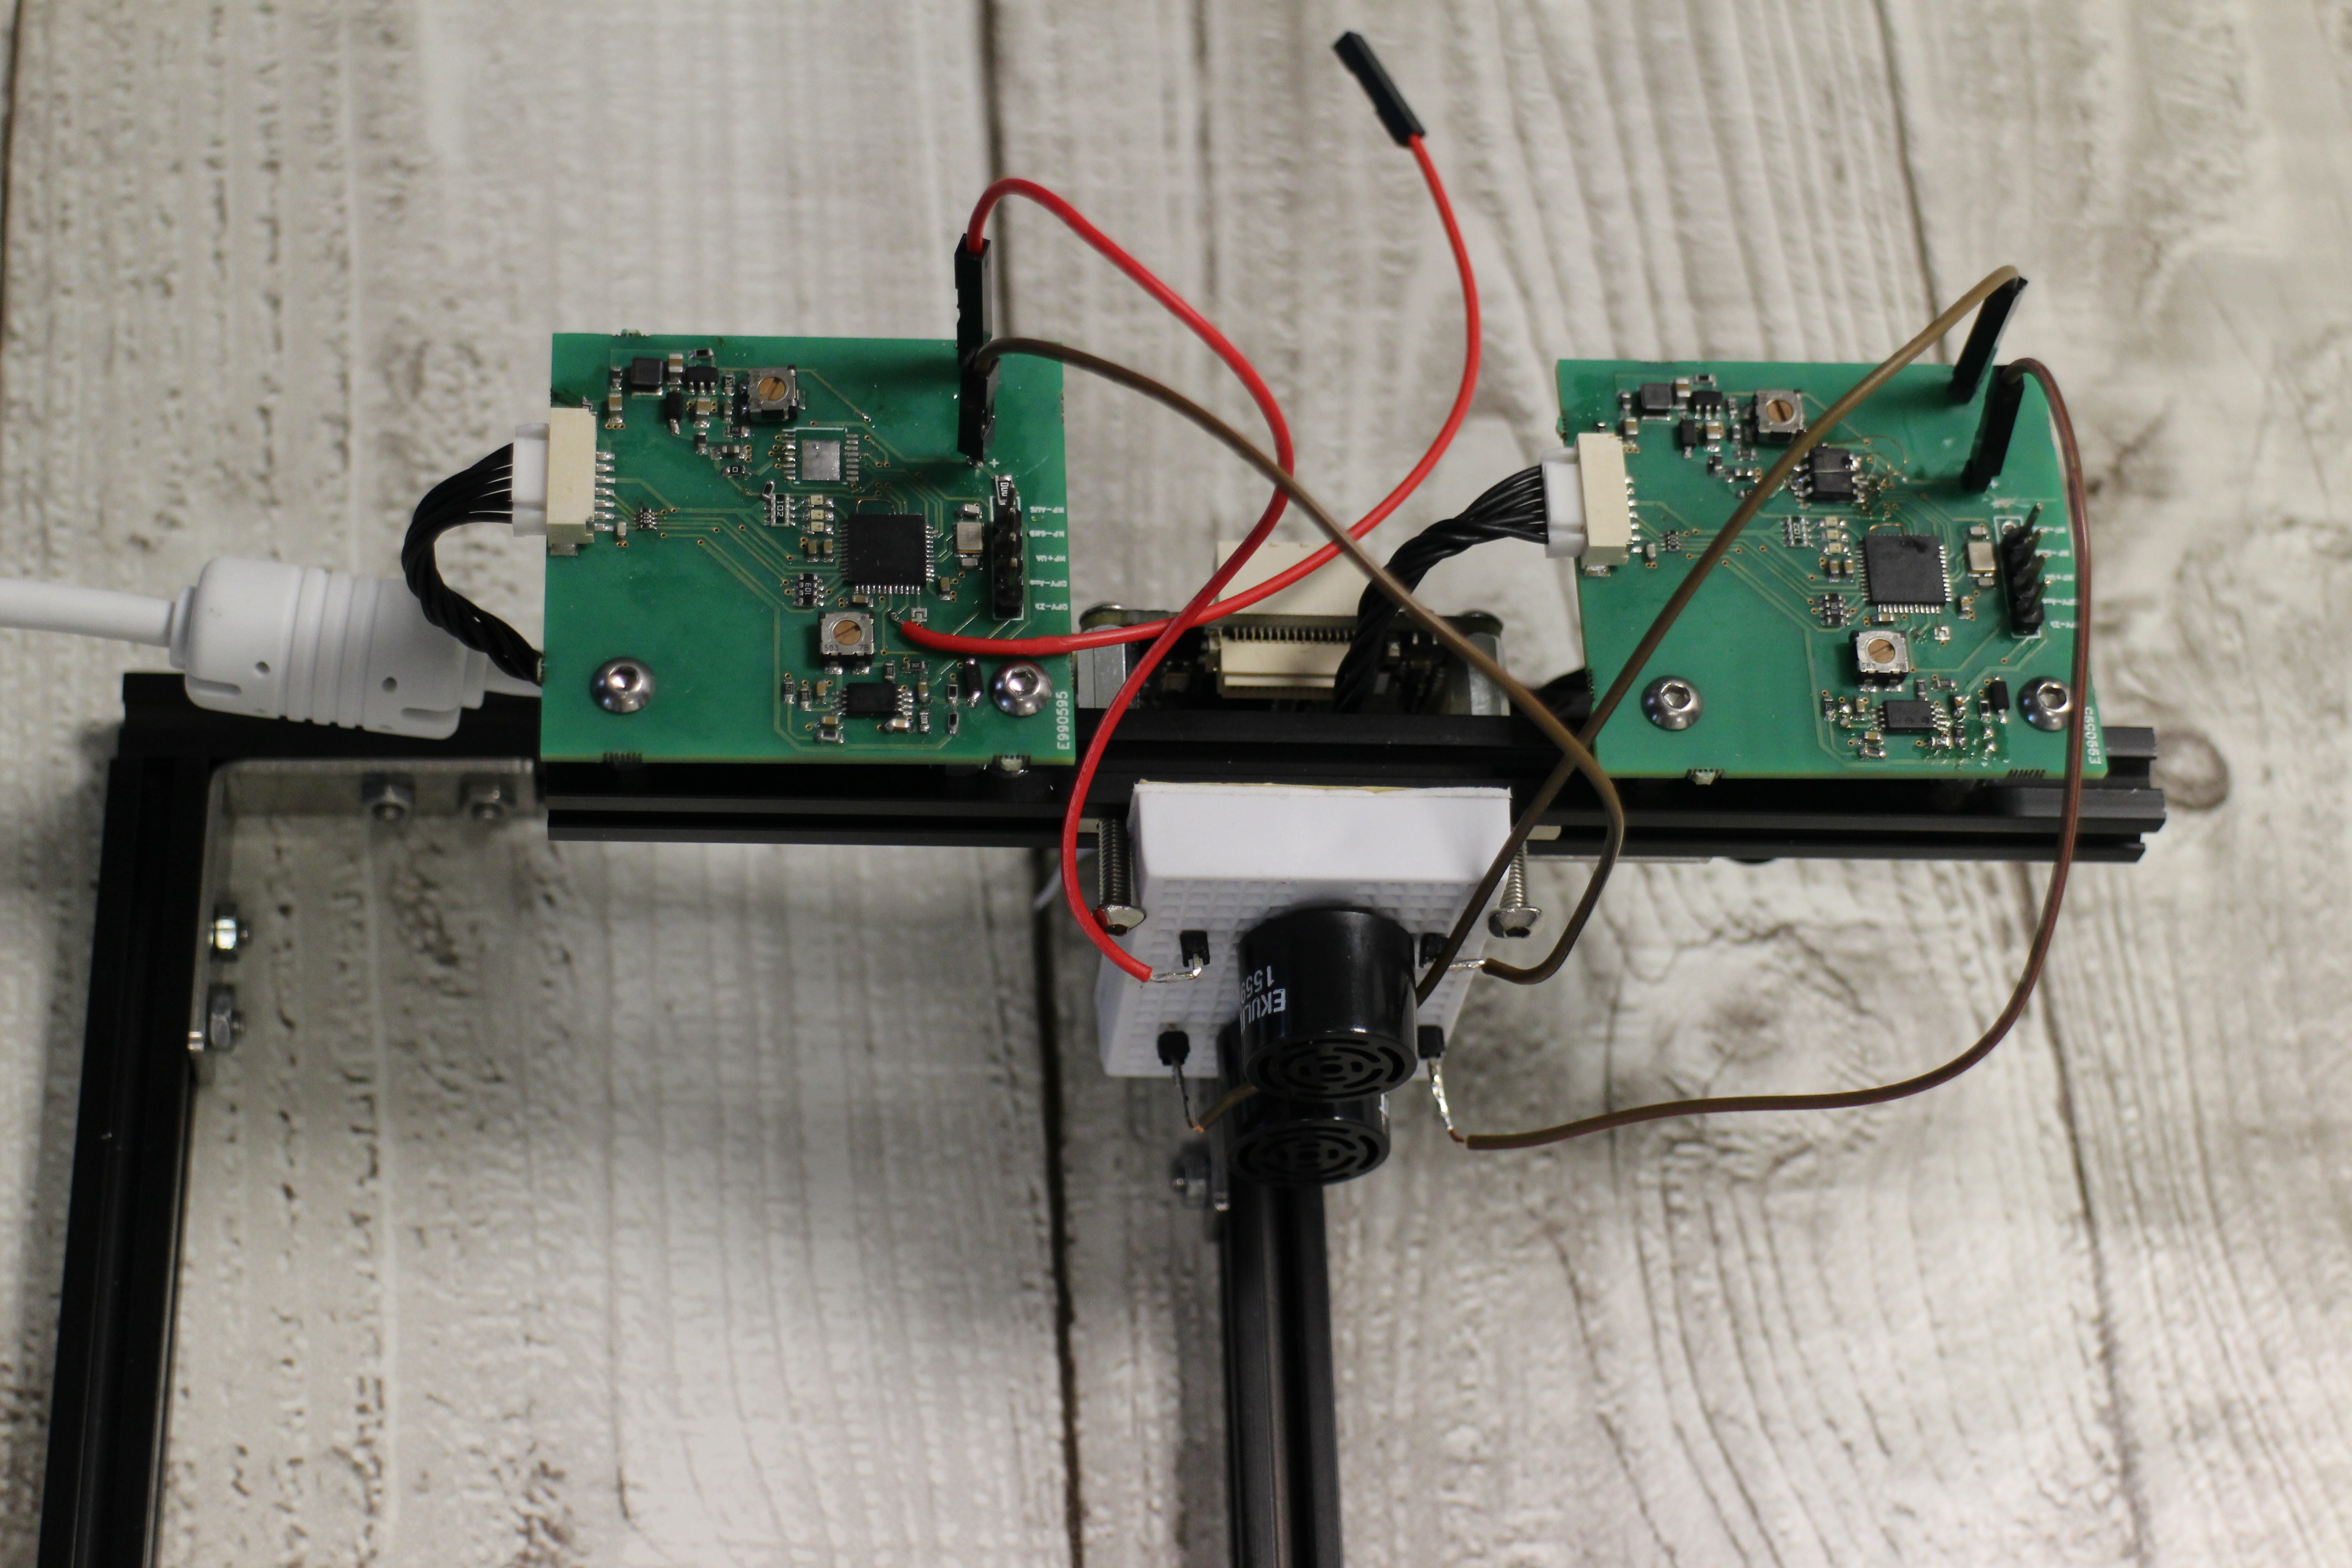
\includegraphics[width=1\textwidth%, draft
]{Abbildungen/BilderPrototypen/Prototyp1.JPG}
\captionof{figure}{Aufgebaute und bearbeitete Platine des ersten Prototypen}
\label{fig:Prototyp1}
\end{minipage}
\end{center}
Bei dem ersten Prototyp wurden die Sendereinheit und die Empfängereinheit auf getrennten Platinen aufgebaut. So bestand die Möglichkeit, den Senderkreis und den Empfängerkreis unabhängig voneinander zu untersuchen, ohne dass sich elektrische Signale der beiden Schaltkreise überlagern konnten. Anfangs wurde für den Senderkreis eine komplette H-Brücke als Schalter verwendet. Allerdings war der Aufbau nicht funktional, da ein Beschaltungsfehler vorhanden war. Dadurch, dass das IC A5950 eine H-Brücke mit integrierter Kontroll-Logik und eigener Spannungspumpe ist, wurde anhand der Schaltweise der Baugruppe festgestellt, dass diese H-Brücke nicht für die Schaltung einsetzbar ist. Denn durch die nicht veränderbare Ansteuerung der beiden Brückenzweige entstand ein Kurzschluss auf der Platine. Um nicht sofort eine neue Platine in Auftrag geben zu müssen, was einiges an Zeit gekostet hätte, wurde das IC ausgelötet. Danach wurde ein MOSFET als HIGH-Side an der Stelle eingesetzt. Vergleiche Abbildung \ref{fig:hiside} Die notwendige Umverdratung wurde mit Fädeldrat durchgeführt. Dadurch ließen sich erste Versuche realisieren, nichtsdestotrotz entsprach das Ergebnis noch nicht den Anforderungen. Deswegen wurde die Beschaltung an dieser Stelle auf eine Halbbrücke erweitert. Damit war die Funktion des Senderkreises für die ersten Versuche und Messungen gegeben.\\
Der Empfängerkreis war von Beginn an funktional, konnte aber erst mit Inbetriebnahme des Senderkreises richtig getestet werden. Am Empfängerkreis wurden zu Testzwecken Änderungen an der Filterung, vor dem Verstärker, vorgenommen. Die Filterung wurde in ihrer Dimensionierung verändert, um herauszufinden, wie sich die Qualität des Echo-Signals verbessern lässt.\\

\begin{minipage}{1\textwidth}
\begin{center}
\includegraphics[width=0.5\textwidth%, draft
]{Abbildungen/h-side.png}
\captionof{figure}{Aufbau des Senders mit einem HIGH-Side}
\label{fig:hiside}
\end{center}
\end{minipage}

\subsection{Senderkreis}
Zuerst wurden Signale direkt an dem Mikrocontroller gemessen, um sicher zu stellen, dass die Einstellungen im Programm die gewünschten Ausgaben zur Folge haben, und keine Gefährdung der Bauteile entsteht.
Um das Signal für die Entfernungsmessung zu generieren wurde der Prozessor so programmiert, dass zehn Impulse mit einer Frequenz von 40\,kHz ausgegeben werden. Danach erfolgt eine Pause, um das zurückkehrende Signal abzuwarten und auszuwerten.\\
\begin{minipage}{0.46\textwidth}
\includegraphics[width=1\textwidth%, draft
]{Abbildungen/MessungenP1/PWM-von-der-cpu.png}
\captionof{figure}{PWM-Burst auf 40\,kHz Basis an der CPU}
\label{fig:pwm-burst}
\end{minipage}\qquad
\begin{minipage}{0.46\textwidth}
\includegraphics[width=1\textwidth%, draft
]{Abbildungen/MessungenP1/PWM-ausgabe-mit-Hi-Side.png}
\captionof{figure}{PWM Ausgabe über einen HIGH-Side}
\label{fig:HiSide}
\end{minipage}\\
In der Abbildung \ref{fig:pwm-burst} ist zu sehen, dass der gewünschte Burst aus zehn Impulsen mit einer Periodendauer von jeweils 25\,\textmu s vom Mikrocontroller generiert wurde. Diese Messung wurde auch vorgenommen, um zu überprüfen, wie das Signal durch die eingesetzten Bauteile verändert wird.\\
Die Abbildung \ref{fig:HiSide} zeigt, wie das Ausgangssignal nach einer HIGH-Side aussah. So wurde zwar im Takt des PWM-Signals geschaltet, allerdings fehlte es an einem Gegenpol, um das Potential in den Schaltpausen wieder auf Null zu ziehen. Somit blieb die Spannung während des Schaltens immer auf einem erhöhten Pegel und sank erst nach Ende des PWM-Signals allmählich ab. Dadurch konnte keine vernünftige Ausgabe an der Ultraschallkapsel erzeugt werden, denn ohne deutliche Potentialunterschiede konnte diese auch nicht in Schwingungen versetzt werden. Der ausgegebene Schalldruck würde nur für kurze Entfernungsmessungen reichen. Das zurückkommende Signal wäre von der abklingenden Spannung des HIGH-Side überlagert worden. Somit war dieser Aufbau nicht umsetzbar.\\
Um die Spannung nicht nur auf einen HIGH-Pegel, sondern auch auf einen LOW-Pegel schalten zu können wurde danach auf eine Halbbrücke gewechselt. Mit dieser ließ sich der Ausgang, über zwei durch das PWM-Signal gesteuerte MOSFETs, sauber auf HIGH- oder LOW-Pegel schalten. 
Mit der verwendeten Halbbrücke ergab sich die Abbildung \ref{fig:Halfbridge}\\
\begin{minipage}{0.46\textwidth}
\includegraphics[width=1\textwidth%, draft
]{Abbildungen/MessungenP1/PWM-Nach-der-Halbbrucke.png}
\captionof{figure}{PWM Ausgabe über eine Halbbrücke}
\label{fig:Halfbridge}
\end{minipage}\qquad
\begin{minipage}{0.46\textwidth}
\includegraphics[width=1\textwidth%, draft
]{Abbildungen/MessungenP1/PWM-Nach-der-Halbbrucke-mit-LS.png}
\captionof{figure}{Ausgabe der PWM an der Ultraschallkapsel}
\label{fig:Senderausgabe}
\end{minipage}\\
Es zeigt sich, dass das Signal nach der Erweiterung auf eine Halbbrücke wieder wie das von dem Mikrocontroller ausgegebene PWM-Signal aussah. Vergleiche Abbildung \ref{fig:pwm-burst}. Die Amplitude fiel wie geplant höher aus. Somit konnte die Höhe der Amplitude über die Spannungspumpe variiert werden um die Stärke des ausgegebenen Signals zu verändern, ohne den Mikrocontroller durch die höhere Spannung zu beschädigen. Wie in der Abbildung \ref{fig:Senderausgabe} zu entnehmen ist, entstanden durch die angeschlossene Ultraschallkapsel höhere Spannungsimpulse in den Schaltmomenten. Diese Spannungsspitzen, die durch die Ultraschallkapsel entstanden, wurden in den Expirementen vernachlässigt, da keine Gefährdung anderer Bauteile entstand. Das dadurch generierte Ausgangssignal entsprach den Anforderungen und musste für die Versuche nicht weiter bearbeitet werden.
\subsection{Empfängerkreis}
Die Platinen des Sender- und Empfängerkreises wurden gemeinsam auf einer Halterung montiert, damit die Ultraschallkapseln zum senden und empfangen der Signale nebeneinander befestigt werden konnten. Ziel war es, durch verschieben eines Hindernisses die Signaländerungen an den Platinen beobachten zu können, ohne die gesamten Messaufbauten bewegen zu müssen. Bei der Aufnahme der Messungen wurde der Empfängerkreis Schritt für Schritt überprüft, um zu erfahren, wie sich das empfangene Signal durch die einzelnen Bauteile verändert.\\
\begin{minipage}{0.46\textwidth}
\includegraphics[width=1\textwidth%, draft
]{Abbildungen/MessungenP1/Signal-Empfang.png}
\captionof{figure}{Signal Empfang}
\label{fig:Empfang am LS}
\end{minipage}\qquad
\begin{minipage}{0.46\textwidth}
\includegraphics[width=1\textwidth%, draft
]{Abbildungen/MessungenP1/Signal-nach-Verstarkung.png}
\captionof{figure}{Signal nach Verstärkung}
\label{fig:Verstaerkung}
\end{minipage}\\
Die Abbildung \ref{fig:Empfang am LS} zeigt das Signal, das direkt am Empfänger zu messen war. Hier waren verschiedene vorerst nicht zuordenbare Signale zu sehen. Allein aus diesem Bild ließ sich daher keine Aussage zu den einzelnen Signalen machen. Fest stand nur, dass ebenfalls Signale die nicht der gewünschten Frequenz entsprachen, vom Empfänger aufgenommen wurden. Dieses Problem galt es natürlich zu beheben, um unerwünschte Störungen zu vermeiden.
Die Abbildungen \ref{fig:Verstaerkung} und \ref{fig:Verstaerkung2} zeigen den Verlauf des Signals nach der Filterung und Verstärkung in zwei verschiedenen Zeitauflösungen. Dabei entspricht \ref{fig:Verstaerkung} den ersten drei Messintervallen von \ref{fig:Verstaerkung2} und dient um darzustellen, dass die Verstärkung eine maximale Aussteuerung von 3,3\,V nicht überschreitet.\\
\begin{minipage}{0.46\textwidth}
\includegraphics[width=1\textwidth%, draft
]{Abbildungen/MessungenP1/Signal-nach-Verstarkung2.png}
\captionof{figure}{Signal nach Verstärkung 2}
\label{fig:Verstaerkung2}
\end{minipage}\qquad
\begin{minipage}{0.46\textwidth}
\includegraphics[width=1\textwidth%, draft
]{Abbildungen/MessungenP1/Signal-nach-Komparator.png}
\captionof{figure}{Signal nach Komparator}
\label{fig:Komparator}
\end{minipage}\\
Nach dem das Signal den Komparator passiert hatte, ergab sich das Bild wie in Abbildung \ref{fig:Komparator} zu sehen ist. Bei einem Vergleich mit dem Signal nach der Verstärkung \ref{fig:Verstaerkung2} wurde sichtbar, dass der Komparator nur Signale, die über seinem Schwellwert von 1,8\,V liegen, durchschaltet. Die Aufteilung in zwei Signalblöcke in den Abbildungen kam daher, dass der erste Block das Signal der Sender-Kapsel ist, das direkt beim Senden seitlich auf die Empfänger-Kapsel abgestrahlt wurde. Der zweite Block ist bereits das Echo, das vom 20\,cm entfernten Hindernis zurückgeworfen wurde.\\
Auch wurden Vergleichsmessungen mit Ultraschallkapseln verschiedener Hersteller durchgeführt. Für die nachfolgenden Abbildungen wurden  Ultraschallkapseln des Herstellers MURATA verwendet. Für Abbildung \ref{fig:MURATAs1,5m} wurden sowohl für den Sendebetrieb, als auch für den Empfängerbetrieb, als Sender deklarierte Ultraschallkapseln verwendet. Für die Abbildung \ref{fig:MURATAsr1,5m} wurden die Kapseln entsprechend der Beschriftung verwendet.\\
\begin{minipage}{0.46\textwidth}
\includegraphics[width=1\textwidth%, draft
]{Abbildungen/MessungenP1/MURATAs1,5m.png}
\captionof{figure}{Betrieb mit zwei Sender-Kapseln}
\label{fig:MURATAs1,5m}
\end{minipage}\qquad
\begin{minipage}{0.46\textwidth}
\includegraphics[width=1\textwidth%, draft
]{Abbildungen/MessungenP1/MURATAsr1,5m.png}
\captionof{figure}{Betrieb mit Sender- und Empfänger-Kapsel}
\label{fig:MURATAsr1,5m}
\end{minipage}\\
Bei Betrachtung der beiden Abbildungen ist zu sehen, dass bei beiden Varianten Signale empfangen wurden. Bei Aufnahme der Abbildung \ref{fig:MURATAs1,5m} war die Empfindlichkeit des Empfängers wesentlich geringer als bei Abbildung \ref{fig:MURATAsr1,5m}. Daraus ergibt sich, dass bei diesem Hersteller die Sender- und die Empfängerkapsel bauliche Unterschiede aufweisen. Aus weiteren Vergleichsmessungen ging hervor, dass die Ultraschallkapseln des Herstellers EKULIT weder vertauscht, noch verpolt werden können. Bei allen Versuchen blieben die Resultate gleich. Demnach gibt es keinen baulichen Unterschiede bei den Sender- und Empfängerkapseln dieses Herstellers.
Anhand der gesammelten Ergebnisse kann festgehalten werden, dass die einfachere Version des Ultraschall-Entfernungsmessers durchaus simpel umzusetzen ist. Es fehlt nur noch ein Programm, das die Zeit zum Eintreffen des Echo-Signals in einen Abstand zum Hindernis konvertiert. Besagtes Programm wurde nicht für diese Prototyp-Version erstellt, da der Anspruch bestand, den Betrieb nicht nur über eine Platine, sondern auch noch über eine einzelne Ultraschallkapsel ablaufen zu lassen.
\newpage
\section{Prototyp 2}
\begin{center}
\begin{minipage}{0.75\textwidth}
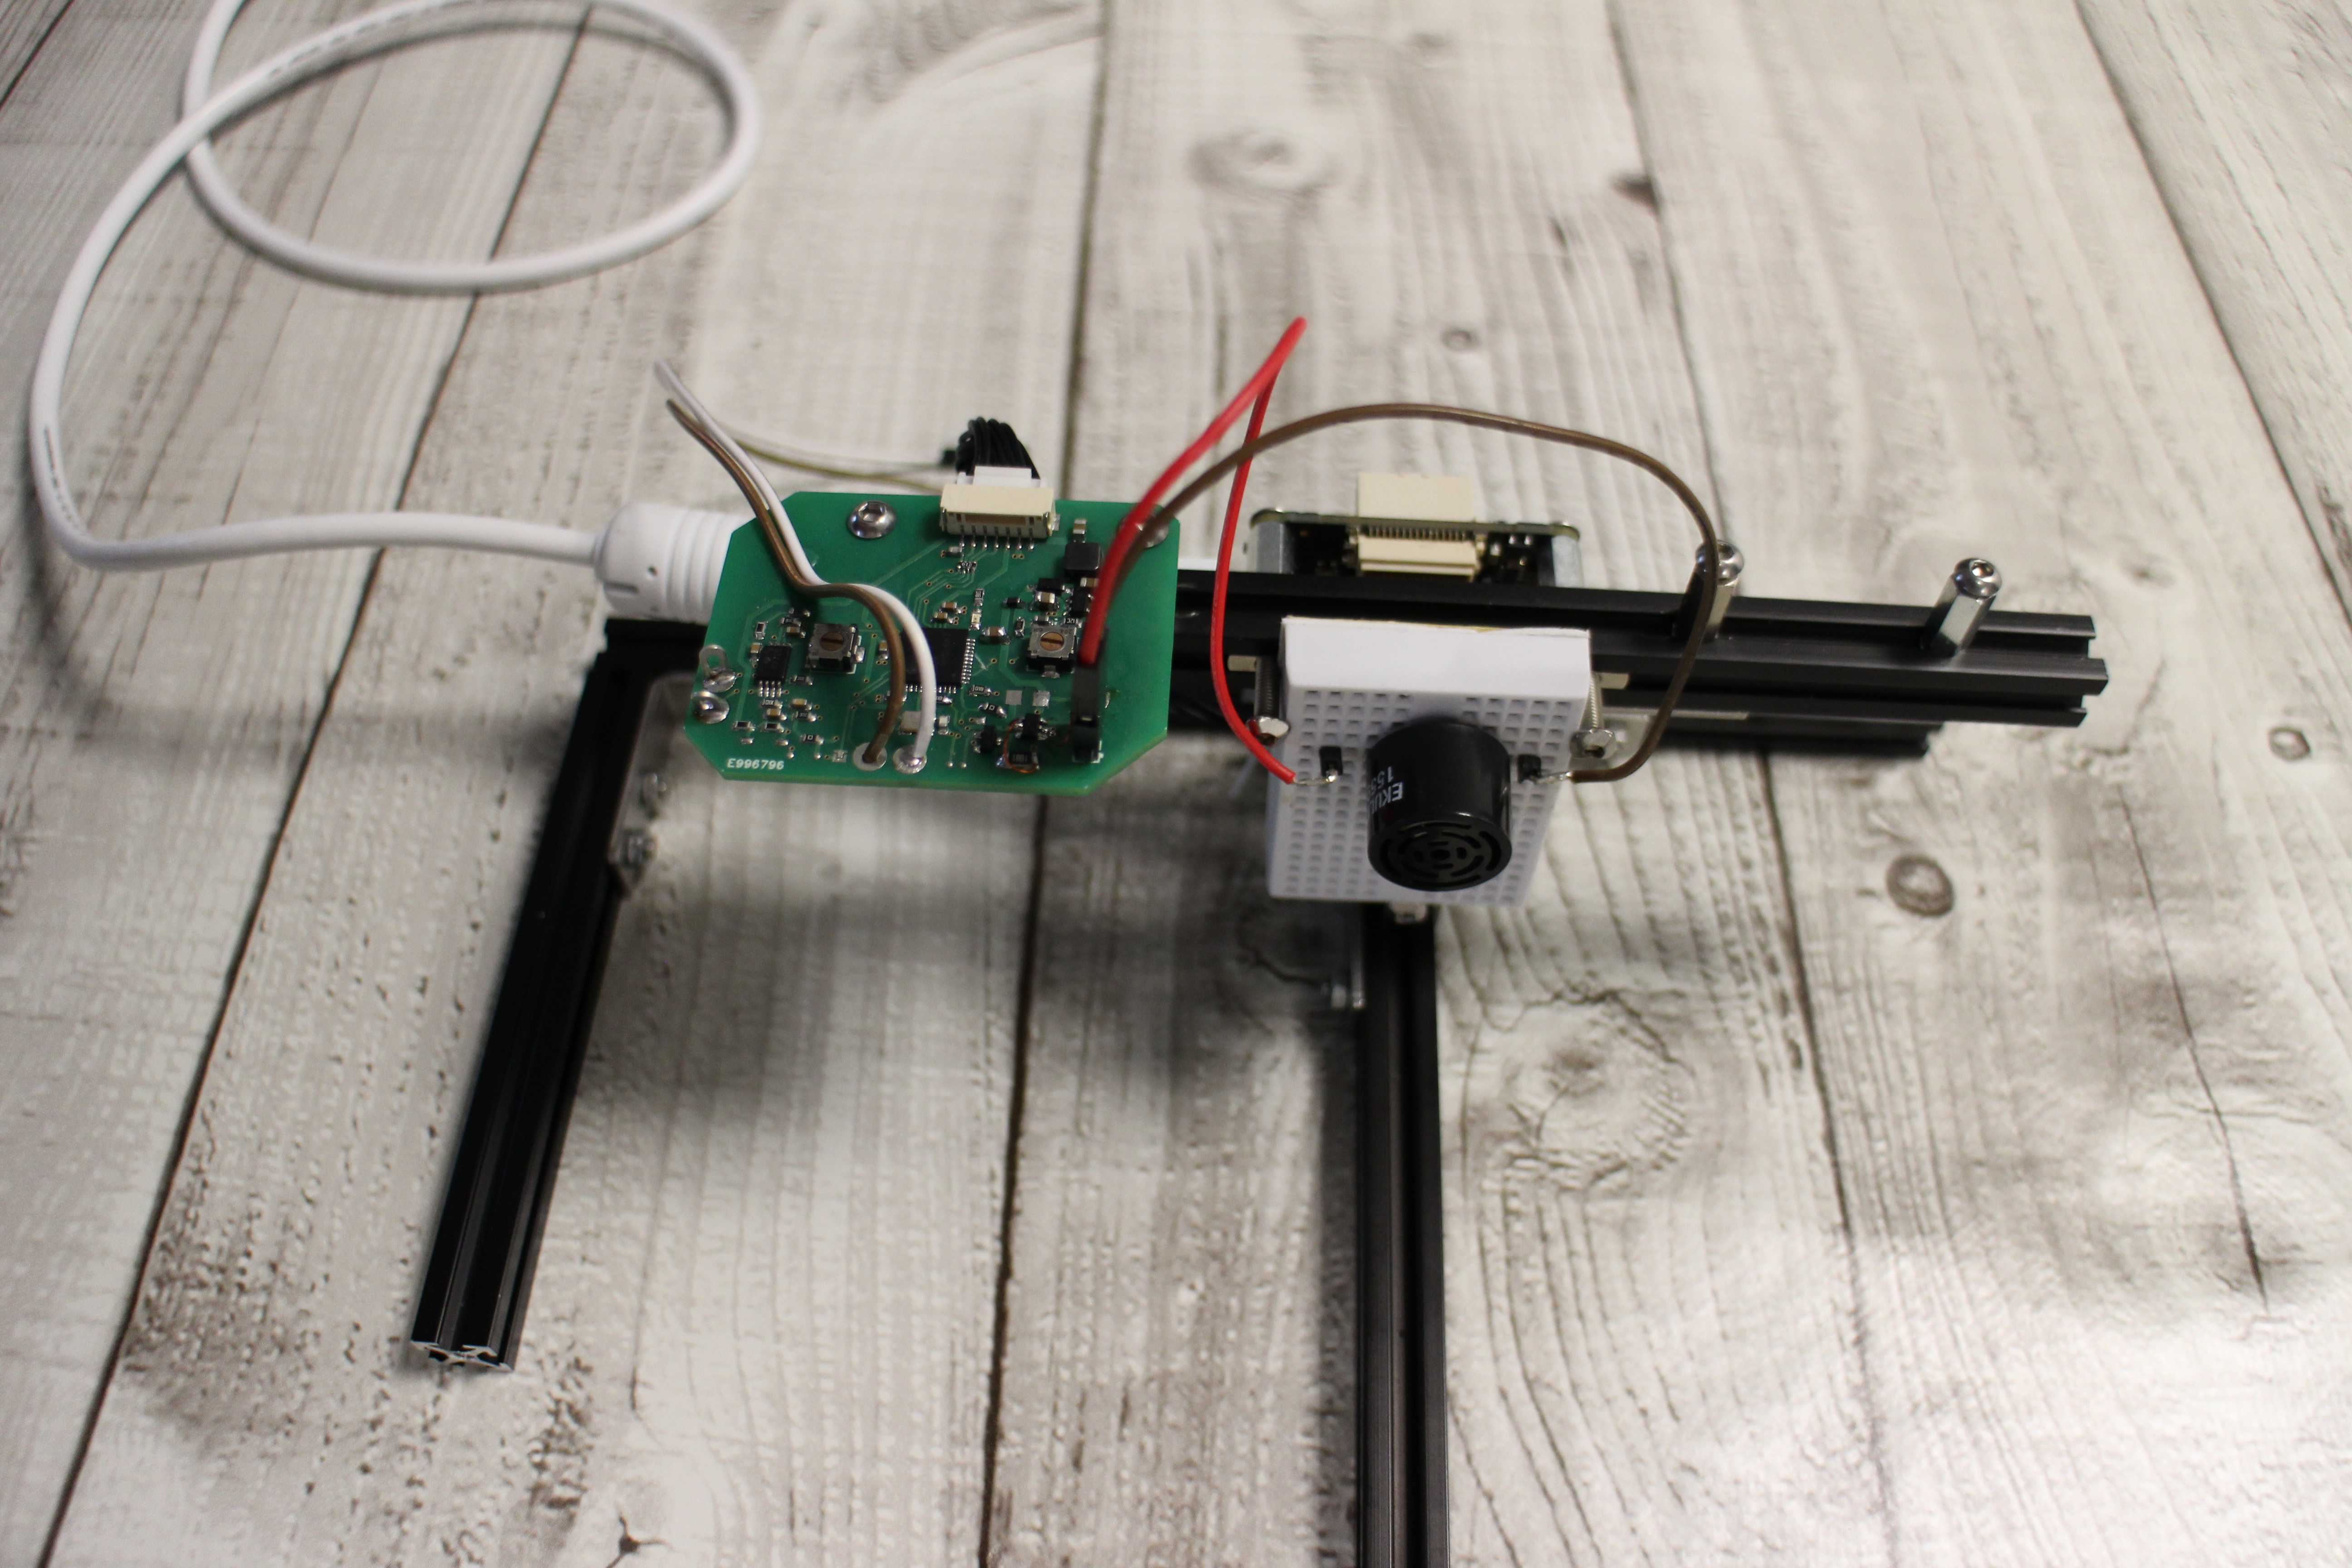
\includegraphics[width=1\textwidth%, draft
]{Abbildungen/BilderPrototypen/Prototyp2.JPG}
\captionof{figure}{Aufgebaute und bearbeitete Platine des zweiten Prototypen}
\label{fig:Prototyp2}
\end{minipage}
\end{center}
Nachdem mit der ersten Prototyp-Version Versuche an der Elektronik durchgeführt wurden und erste Messungen mit einem beweglichen Hindernis auswertbare Ergebnisse brachten, wurde eine zweite Prototyp-Version entworfen. Bei der zweiten Prototyp-Version wurden der Sender- und der Empfängerkreis auf einer Platine aufgebaut und es wurde nur noch eine Ultraschallkapsel für beide Anwendungen vorgesehen. Dadurch musste die Halbbrücke, für den fehlerfreien Betrieb, drei und nicht zwei Schaltzustände haben. Deswegen wurde die Halbbrücke der ersten Prototyp-Version durch eine voll gesteuerte Halbbrücke ersetzt. Nicht nur sollte die Ultraschallkapsel mit HIGH-, oder LOW-Signal steuerbar sein, auch ein dritter potentialfreier Zustand war nötig. Nur so konnten die Echo-Signale auch empfangen werden. Hinzu kommt, dass durch den neuen Platinenentwurf Verbesserungen, die ab der ersten Prototyp-Version vorgenommen wurden, direkt in den Schaltplan übernommen werden konnten. Dadurch ließ sich die Störanfälligkeit durch empfindliche Drahtbrücken deutlich reduzieren. Bedingt durch anfängliche Befürchtungen wurden für die MOSFETs der Halbbrücke anfangs ein weiteres MOSFET\,(Q\textsubscript{2}) eingesetzt. Dieser Zusatz stellte sich als unnötig heraus, da die zusätzliche Sicherheit, die das Bauteil mit sich bringen sollte, überflüssig war. Somit wurde das überflüssige MOSFET\,(Q\textsubscript{2}) entfernt. Die Beschaltung ist in der Abbildung \ref{fig:halbbrücke} einzusehen. Durch zwei Drahtbrücken konnte die komplette Schaltung nach Behebung eines weiteren Verdrahtungsfehlers, in Betrieb genommen werden.\\
\begin{center}
\begin{minipage}{0.75\textwidth}
\includegraphics[width=1\textwidth%, draft
]{Abbildungen/halbbrucke.png}
\captionof{figure}{Aufbau der Halbbrücke mit vier MOSFETs, Q\textsubscript{2} und R\textsubscript{21} wurden für den weiteren Betrieb entfernt}
\label{fig:halbbrücke}
\end{minipage}
\end{center}
Um bei diesem Aufbau einen fehlerfreien Betrieb der verwendeten voll gesteuerten Halbbrücke sicherzustellen, wurden durch den Mikrocontroller zwei ineinander verschachtelte PWM-Signale generiert. Diese sind wie in der Abbildung \ref{fig:PWMs} zu sehen ist durch kleine Lücken getrennt. Verzögerungen im Schaltbetrieb der Halbleiter konnten daher, keine Kurzschlüsse mehr verursachen.\\
\begin{center}
\begin{minipage}{0.75\textwidth}
\includegraphics[width=1\textwidth%, draft
]{Abbildungen/MessungenP2/Zwei_PWMs_von_der_CPU.PNG}
\captionof{figure}{Verlauf der zwei generierten PWMs für den Betrieb der voll gesteuerte Halbbrücke}
\label{fig:PWMs}
\end{minipage}\\
\end{center}
Nachdem dieser Betrieb sichergestellt war, wurden Messungen am Verstärker (obere Linie), und am Komparator (untere Linie) vorgenommen. Dabei wurde die Verstärkung so eingestellt, dass unerwünschte Störungen nicht vom Komparator weitergegeben wurden. Die Spannung für den Sendebetrieb wurde für die Versuche zwischen 5\,V und 20\,V variiert, um betrachten zu können, wie sich das auf die Reichweite und Genauigkeit der Messungen auswirkt. Als Hindernis wurde bei allen Experimenten eine glatte Holzplatte der Maße 50x64\,cm verwendet und in einem Abstand von ein bis fünf Metern von der Ultraschallkapsel entfernt aufgestellt. In den Abbildungen \ref{fig:5v1m} bis \ref{fig:5v4m} sind die Ergebnisse einer Messreihe mit einer Spannung von 5\,V für den Sendebetrieb dargestellt. Die Ansicht wurde so eingestellt, dass zwei Sendeimpulse zu sehen sind. Dadurch wird deutlicher, welches die Sende Impulse sind, und welches die von der Entfernung abhängigen Echos sind.\\
\begin{minipage}{0.46\textwidth}
\includegraphics[width=1\textwidth%, draft
]{Abbildungen/MessungenP2/5V/1mb.PNG}
\captionof{figure}{Signalverlauf bei 5\,V auf 1\,m Abstand}
\label{fig:5v1m}
\end{minipage}\qquad
\begin{minipage}{0.46\textwidth}
\includegraphics[width=1\textwidth%, draft
]{Abbildungen/MessungenP2/5V/2mb.PNG}
\captionof{figure}{Signalverlauf bei 5\,V auf 2\,m Abstand}
\label{fig:5v2m}
\end{minipage}\\
\begin{minipage}{0.46\textwidth}
\includegraphics[width=1\textwidth%, draft
]{Abbildungen/MessungenP2/5V/3mb.PNG}
\captionof{figure}{Signalverlauf bei 5\,V auf 3\,m Abstand}
\label{fig:5v3m}
\end{minipage}\qquad
\begin{minipage}{0.46\textwidth}
\includegraphics[width=1\textwidth%, draft
]{Abbildungen/MessungenP2/5V/4mb.PNG}
\captionof{figure}{Signalverlauf bei 5\,V auf 4\,m Abstand}
\label{fig:5v4m}
\end{minipage}\\
Bei den Abbildungen ist zu sehen, dass das Echo-Signal mit zunehmender Entfernung immer schwächer wird. Bei einer Entfernung von vier Metern (Abbildung \ref{fig:5v4m}) wird das Echo-Signal so schwach, dass die Signalstärke nach dem Komparator nicht mehr für eine eindeutige Auswertung über den Mikrocontroller ausreicht. Nachfolgend sind die Abbildungen einer Messreihe mit verschiedenen Spannungseinstellungen für den Sendebetrieb zu sehen. Anhand dieser Messreihe soll dargestellt werden, welchen Einfluss die eingestellte Spannung im Sendebetrieb auf die Reichweite des Ultraschallsignals hat. Für die Darstellung wurden die Messungen bei 5 Meter Abstand ausgewählt.\\
\begin{minipage}{0.46\textwidth}
\includegraphics[width=1\textwidth%, draft
]{Abbildungen/MessungenP2/5V/5m.PNG}
\captionof{figure}{Signalverlauf bei 5\,V auf 5\,m Abstand}
\label{fig:5v5m2}
\end{minipage}\qquad
\begin{minipage}{0.46\textwidth}
\includegraphics[width=1\textwidth%, draft
]{Abbildungen/MessungenP2/10V/5mb.PNG}
\captionof{figure}{Signalverlauf bei 10\,V auf 5\,m Abstand}
\label{fig:10v5m}
\end{minipage}\\
\begin{minipage}{0.46\textwidth}
\includegraphics[width=1\textwidth%, draft
]{Abbildungen/MessungenP2/15V/5mb.PNG}
\captionof{figure}{Signalverlauf bei 15\,V auf 5\,m Abstand}
\label{fig:15v5m}
\end{minipage}\qquad
\begin{minipage}{0.46\textwidth}
\includegraphics[width=1\textwidth%, draft
]{Abbildungen/MessungenP2/20V/5mb.PNG}
\captionof{figure}{Signalverlauf bei 20\,V auf 5\,m Abstand}
\label{fig:20v5m}
\end{minipage}\\
Beim Vergleich der Abbildungen \ref{fig:5v5m2} und \ref{fig:10v5m} mit den Abbildungen \ref{fig:15v5m} und \ref{fig:20v5m}  ist zu sehen, dass bei einem Abstand von 5 Metern erst bei einer Sendespannung von über 10\,V, auch am Komparator ein für den Mikrocontroller auswertbares Signal vorhanden ist. Dies bedeutet, dass Entfernungsmessungen auf eine kurze Distanz zwar mit der vorhandenen Versorgungsspannung von 5\,V realisierbar sind. Soll die Reichweite aber über vier Meter betragen, so ist eine Erhöhung der Sendespannung notwendig. Auch die Signalverläufe mit einer Sendespannung von 20\,V wurden bei Entfernungen von über fünf Metern deutlich schwächer. So ließ sich mit vierfacher Sendespannung nicht einmal die doppelte Reichweite realisieren. Messungen auf sechs Meter Abstand brachten keine eindeutigen Ergebnisse hervor.\\
In der nachfolgenden Tabelle \ref{tab:Entfernungsmessung} wurden die Zeitabstände vom ersten Impuls des gesendeten Signals, bis zum ersten Impuls des Echo-Signals aufgetragen. Anhand der Schallgeschwindigkeit die Entfernung, die der Schall zurückgelegt hat berechnet. Dazu wurde noch die Abweichung der berechneten Entfernung von der eingestellten Entfernung angegeben.\\


\begin{minipage}{1\textwidth}
\captionof{table}{Entfernungsmessung mit Abweichung bei 20~V Sendespannung}
\begin{tabularx}{\textwidth}{|p{0.17\textwidth}|p{0.27\textwidth}|p{0.27\textwidth}|X|}
\hline
Entfernung [m]& Zeit bis Anfang Echo [ms]  & Errechnete Entfernung [m] & Abweichung [cm]\\
\hline
1 & 6,07 & 1,0416 & 4,16\\
\hline
1,5 & 8,97 & 1,5392 & 3,92\\
\hline
2 & 11,92 & 2,0454 & 4,54\\
\hline
2,5 & 14,8 & 2,5396 & 3,96\\
\hline
3 & 17,75 & 3,0459 & 4,59\\
\hline
3,5 & 20,65 & 3,5435 & 4,35\\
\hline
4 & 23,56 & 4,0428 & 4,28\\
\hline
4,5 & 26,49 & 4,5456 & 4,56\\
\hline
5 & 29,46 & 5,0553 & 5,53\\
\hline
\end{tabularx}

\label{tab:Entfernungsmessung}
\end{minipage}\\


Wie zu erwarten war, sind bei der errechneten Entfernung Abweichungen im Bereich weniger Zentimeter aufgetreten. Bei Betrachtung der Abweichungen wird deutlich, dass die Werte bis auf einen, alle im Bereich von 4\,cm bis 4,5\,cm liegen. Ähnliche Abweichungen waren auch bei den anderen Messreihen zu beobachten. Somit ließe sich die Abweichung durch einen Korrekturwert auf ein Minimum reduzieren und würde einen Zentimeter nur noch selten überschreiten. Den erste Impuls des Echo-Signals als Referenz für die Entfernungsberechnung zu nutzen ist die bessere Wahl. Denn die anfänglichen Überlegungen, den letzten Impuls des Echo-Signals, oder einen Mittelwert aus allen empfangenen Impulsen zu verwenden beinhaltet ein höheres Fehlerpotential. Die Dauer des Echo-Signals kann durch niederfrequente Nebengeräusche deutlich verlängert werden. Dies ließ sich bei einem der Tests beobachten, als im Hintergrund ein Lasercutter betrieben wurde. Dabei entstanden entgegen der Befürchtung keine Störsignale, stattdessen war die Signalintensität des Echo-Signals deutlich höher als bei Versuchen in einer ruhigen Umgebung. 












